\documentclass{beamer}

% Encoding & language
\usepackage[T1]{fontenc}
\usepackage[utf8]{inputenc}
\usepackage[english]{babel}
\usepackage{transparent}

% Bibliography
\usepackage[numbers]{natbib}
\bibliographystyle{ieeetr}

% Figures, tables, colors
\usepackage{graphicx}
\usepackage{subcaption}
\usepackage{tabularx}
\usepackage{booktabs}
\usepackage{multirow}
\usepackage{makecell}
\usepackage[table, svgnames]{xcolor}

\usepackage{caption}
\captionsetup[table]{justification=centering}

% Beamer
\setbeamerfont{framesubtitle}{size=\normalsize}

% Misc
\usepackage{amsmath}
\usepackage{amssymb}
\usepackage{hyperref}
\usepackage{tikz}
\usetikzlibrary{arrows.meta, positioning, calc}
\DeclareMathOperator{\jinc}{jinc}

% Section.slide numbering in frame titles (e.g. "2.3")
\newcounter{sframe}[section]
\renewcommand{\thesframe}{\thesection.\arabic{sframe}}
\newcommand{\ftitle}[1]{\stepcounter{sframe}{\normalsize\thesframe}\quad #1}

% Transparent, Checkmark
\usepackage{transparent}
\newcommand{\dimtxt}[1]{{\transparent{0.25}#1}} % 0.25-0.45
\usepackage{pifont}
\newcommand{\cmark}{\ding{51}}
\newcommand{\xmark}{\ding{55}}

\mode<presentation>{
  \usetheme{Madrid}
  \usecolortheme{default}
  \setbeamertemplate{caption}[numbered]
}

\title[Solar Radio Interferometer Simulation]{%
  {\Large\bfseries End-to-End Simulation of a Four-Element UHF Radio\\
  Interferometer for Solar Radio Observation at 610~MHz}%
}

\subtitle{Graduation Thesis Defense}

\author[N. B. Quan]
{Nguyen Ba Quan (20224350) \\ Supervisor: Assoc.\ Prof.\ Dr.\ Ha Duyen Trung}

\institute[SEEE--HUST]
{
School of Electrical and Electronic Engineering \\
Hanoi University of Science and Technology
}

\date{\today}

\setbeamertemplate{bibliography item}{\insertbiblabel}

\begin{document}

% ============================================================
% Title
\begin{frame}
  \titlepage
\end{frame}

\begin{frame}{Outline}
\tableofcontents
\end{frame}

% ============================================================
\section{Motivation}

\begin{frame}{\ftitle{Problem and Motivation}}
\begin{columns}[c]
\column{.44\textwidth}
\begin{enumerate}
  \item \textbf{2022 Starlink incident:} 38/49 satellites lost to a
  geomagnetic storm~\cite{berger2023starlink}.
  \item Solar radio bursts perturb the ionosphere, degrading
  \textbf{GNSS} positioning accuracy.
  \item Ground-based radio monitoring gives \textbf{early warning} of
  these space-weather events.
\end{enumerate}
\column{.52\textwidth}
\centering
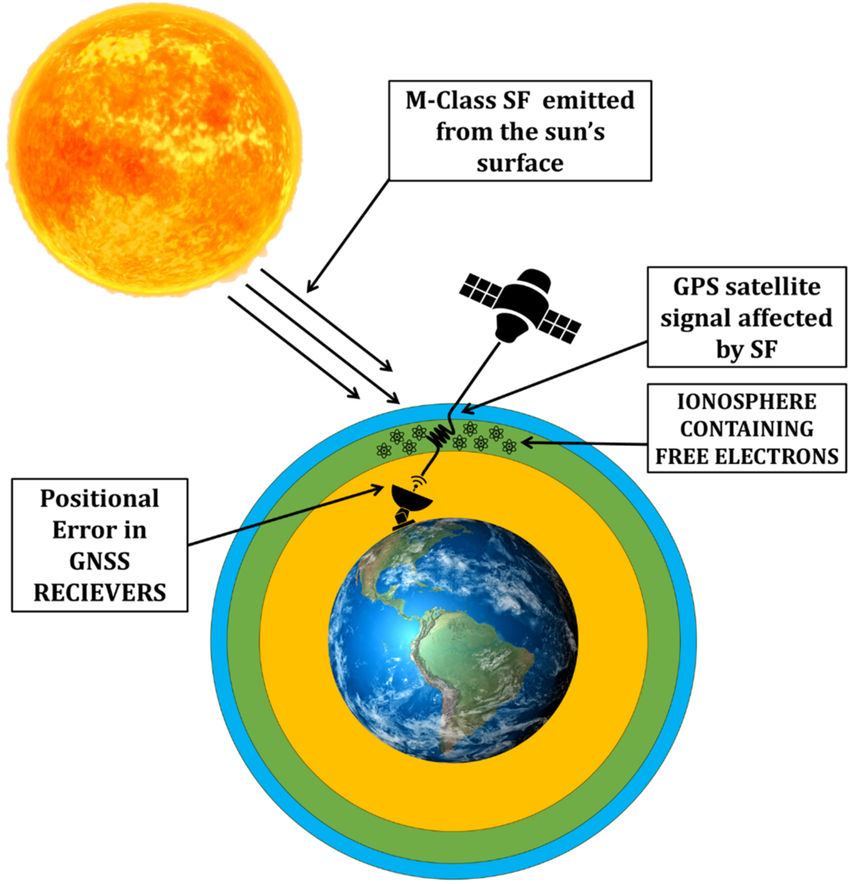
\includegraphics[width=\linewidth]{figs/fig_gnss_ionosphere.png}
\end{columns}
\vspace{4pt}
\centering
\small Fig.~1. How solar radio bursts affect our electronic devices.
\end{frame}

\begin{frame}{\ftitle{Big Dish vs.\ Aperture Synthesis}}
\begin{columns}[t]
\column{.48\textwidth}
\centering
\textbf{Big Parabolic Antenna}\\{\footnotesize (Traditional interferometry)}\\[3pt]
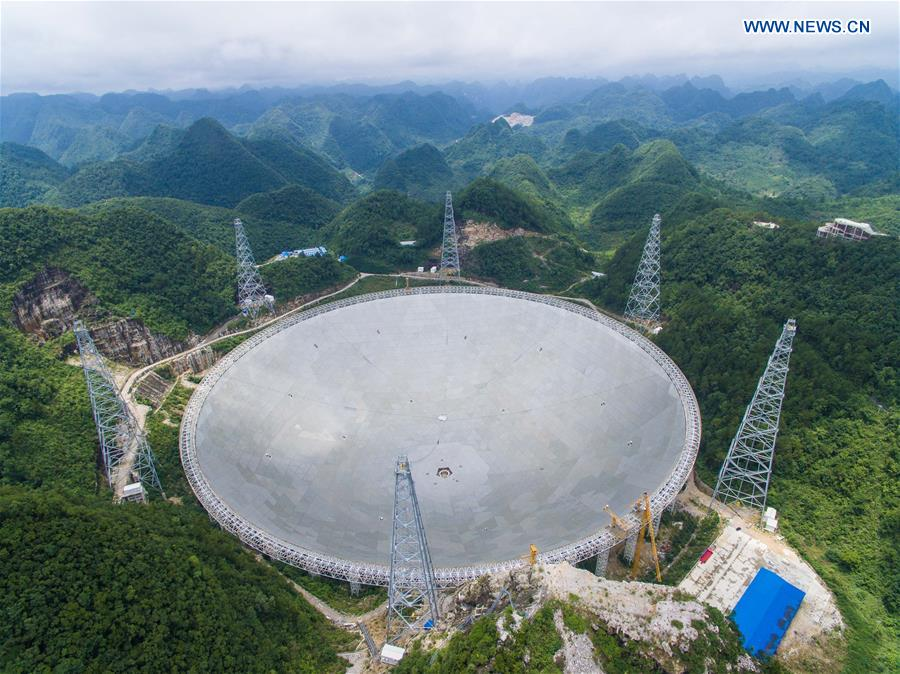
\includegraphics[width=.7\linewidth]{figs/photo_fast_dish.jpg}\\
\footnotesize Fig.~2. 500~m diameter parabolic antenna (FAST, China).
\vspace{3pt}
\begin{itemize}
  \footnotesize
  \item Resolution depends on antenna \textbf{aperture} (biggest today
  $\approx500$~m).
  \item Cost: \textbf{millions of dollars} of infrastructure.
\end{itemize}
\column{.48\textwidth}
\centering
\textbf{Aperture Synthesis}\\{\footnotesize (New concept)}\\[3pt]
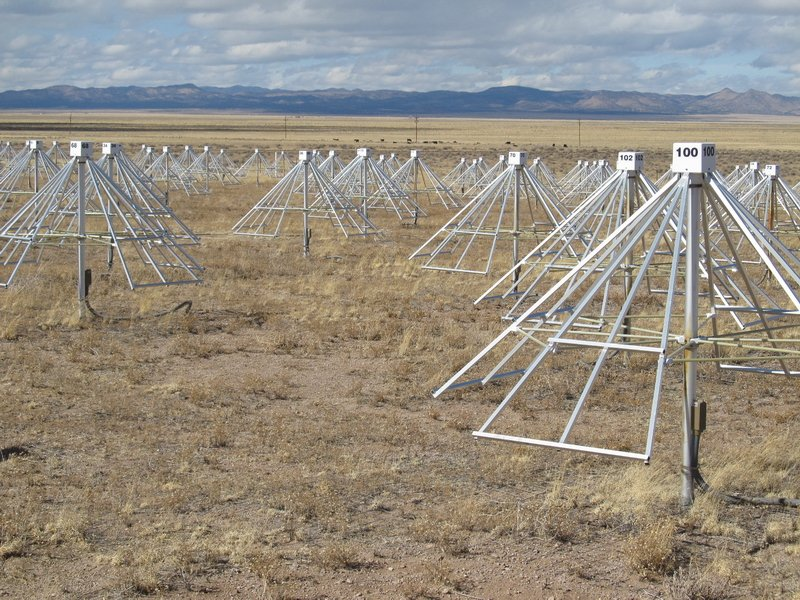
\includegraphics[width=.7\linewidth]{figs/photo_dlite_array.jpg}\\
\footnotesize Fig.~3. DLITE station in the USA, 32 LWA antennas.
\vspace{3pt}
\begin{itemize}
  \footnotesize
  \item Resolution depends on the biggest \textbf{baseline} between
  antennas (thousands of m).
  \item Cost scales with antenna count --- \textbf{thousands of
  dollars} each, many frequencies possible.
\end{itemize}
\end{columns}
\end{frame}

\begin{frame}{\ftitle{The Black-Box Problem}}
\begin{columns}[c]
\column{.44\textwidth}
\textbf{Previous physical deployment}
\begin{itemize}
  \small
  \item Result: only an \textbf{ambiguous day/night trend} --- no clear
  interference fringes.
  \item Four candidate causes:
\end{itemize}
\begin{itemize}
  \footnotesize
  \item[$\square$] Phase-incoherent SDR oscillators?
  \item[$\square$] Cable insertion loss?
  \item[$\square$] Local RFI?
  \item[$\square$] Thermal noise floor too high?
\end{itemize}
\column{.5\textwidth}
\centering
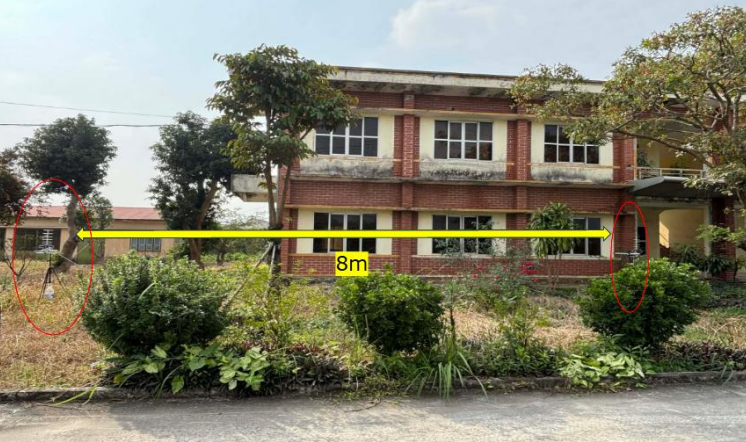
\includegraphics[width=\linewidth]{figs/photo_xuan_mai_field.png}\\
\small Fig.~4. Xuan Mai field trial: 2-element Yagi-Uda, 8~m baseline.
\end{columns}
\vspace{6pt}
\begin{alertblock}{Insight}
\small A hardware black box cannot be debugged by observing and fixing
it blindly. We must build a physically grounded simulation to separate
and quantify these effects \textbf{before} further expensive hardware
deployment.
\end{alertblock}
\end{frame}

\begin{frame}{\ftitle{Objectives}}
\centering
\textbf{This thesis came out to answer two main ideas}
\vspace{10pt}

\begin{columns}[t]
\column{.48\textwidth}
\centering
\textbf{Build a trustworthy\\physics simulation}
\vspace{6pt}

\footnotesize Signal $\to$ correlator $\to$ image. Validated against
classical theory and real hardware, so it can safely stand in before
expensive field testing.
\column{.48\textwidth}
\centering
\textbf{Optimize antenna placement\\(array geometry)}
\vspace{6pt}

\footnotesize Use that simulator to search many array layouts. Find
which placement of the same antennas gives the best 2-D resolution,
without buying more hardware.
\end{columns}
\vspace{14pt}
\centering
\textbf{$\Rightarrow$ Every result in this talk answers one of these two
questions.}
\end{frame}

% ============================================================
\section{Theoretical Background}

\begin{frame}{\ftitle{Solar Radio Bursts: Types I--V}}
\begin{columns}[c]
\column{.55\textwidth}
\begin{itemize}
  \footnotesize
  \item Superimposed on the quiet-Sun thermal background, transient bursts can
  raise the flux by \textbf{orders of magnitude}.
  \item \textbf{Type I}: long-lived, narrowband noise storms.
  \item \textbf{Type III}: fast-drifting, electron beams on open field lines
  --- dominant at decimetre wavelengths.
  \item \textbf{Type II}: slowly drifting, traces coronal shock fronts (CMEs).
  \item \textbf{Type IV}: broadband continuum following flares.
  \item \textbf{Type V}: brief continuum sometimes following Type~III
  bursts, tracing trapped electron streams.
\end{itemize}
\column{.45\textwidth}
\centering
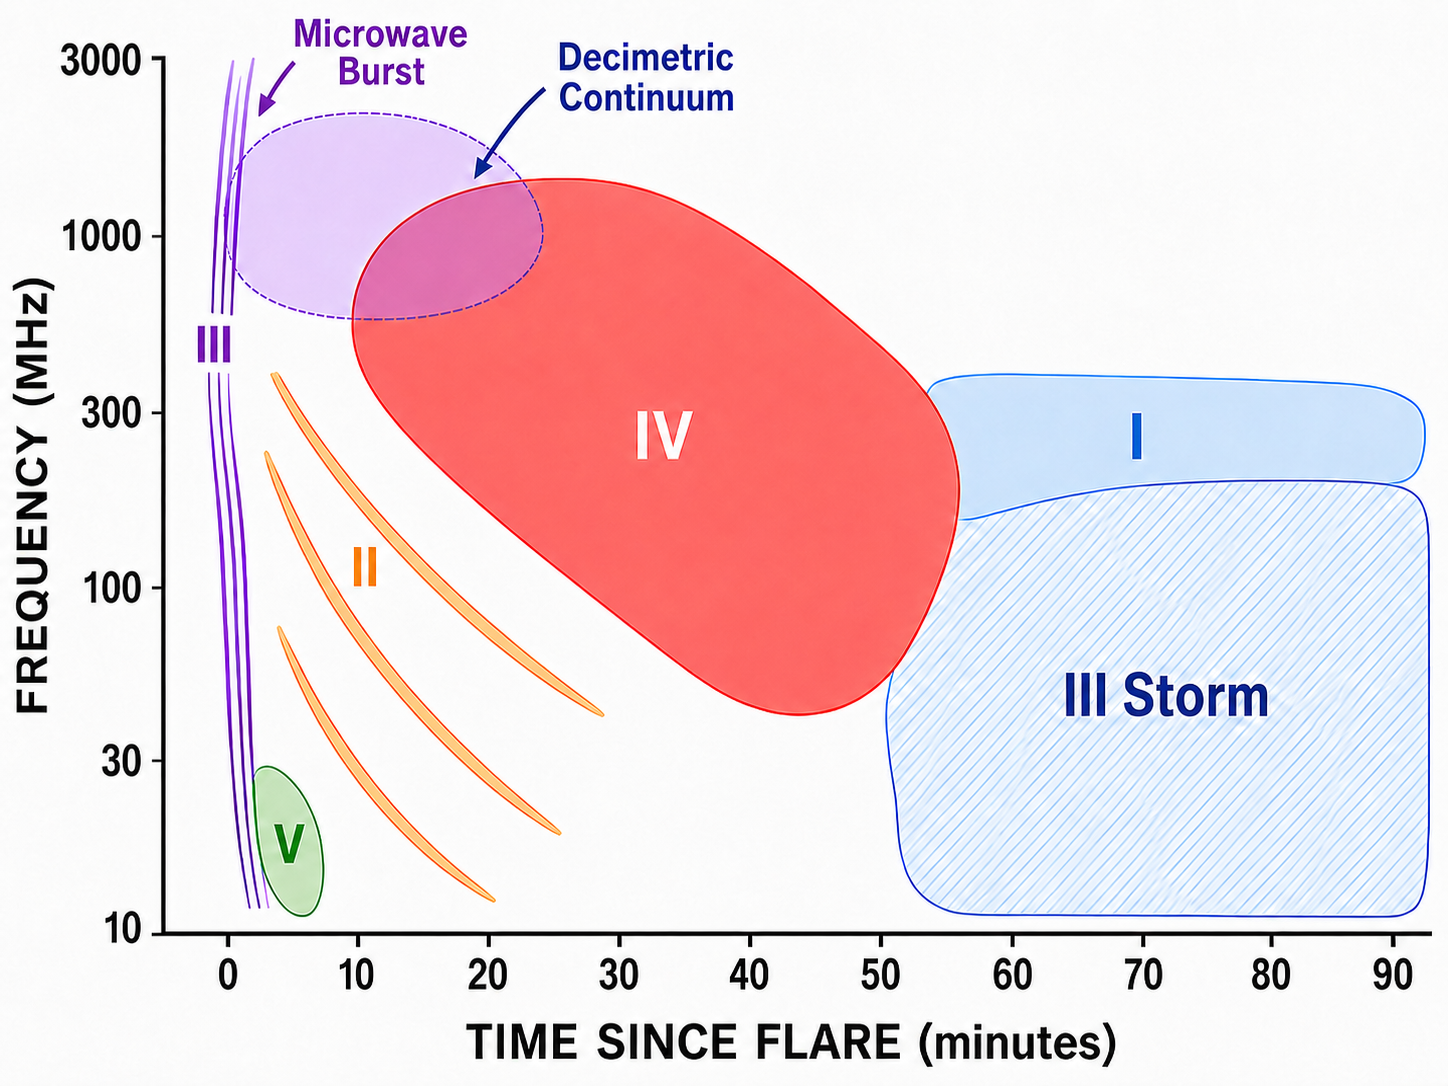
\includegraphics[width=\linewidth]{figs/fig_solar_dynamic_spectrum.png}
\end{columns}
\vspace{4pt}
\small Adapted from McLean \& Labrum and Dulk~\cite{dulk1985}.
\end{frame}

\begin{frame}{\ftitle{Key Formula 1: From Flux to Voltage (Friis)}}
\textbf{Wavelength:} $\lambda = c/f \approx 0.49$~m at 610~MHz.
\vspace{6pt}

\textbf{Friis reception relation:}
\[
P_{\rm sig} = \tfrac{1}{2} A_e\, S_\nu\, \Delta\nu, \qquad A_e = \frac{\lambda^2 G}{4\pi}
\]
\begin{itemize}
  \item $S_\nu$: incident flux density (solar flux units, sfu)~\cite{friis1946}
  \item $A_e$: antenna effective aperture, from the simulated gain $G$
  \item Received power is converted to an equivalent voltage:
  $V_{\rm rms} = \sqrt{P_{\rm rx} R_{\rm load}}$
  \item[$\Rightarrow$] This is the first link of the pipeline: real flux
  in, per-antenna voltage out.
\end{itemize}
\end{frame}

\begin{frame}{\ftitle{Key Formula 2: Receiver Noise (Johnson--Nyquist)}}
\textbf{Johnson-Nyquist thermal noise:}
\[
P_n = k_B\, T_{\rm sys}\, \Delta\nu
\]
\textbf{Radiometer equation:}
\[
\mathrm{SNR} \;\propto\; \sqrt{N_s} \;=\; \sqrt{\Delta\nu\,\tau}
\]
\begin{itemize}
  \item Every receiver adds unavoidable thermal noise~\cite{nyquist1928}, set
  by the system temperature $T_{\rm sys}$.
  \item Averaging $N_s$ samples (integration time $\tau$) improves SNR ---
  the basis for detecting a weak solar signal in noise.
  \item[$\Rightarrow$] This noise term is injected alongside the Friis
  voltage in the simulation pipeline.
\end{itemize}
\end{frame}

\begin{frame}{\ftitle{Key Formula 3: Correlator \& van Cittert--Zernike}}
\centering
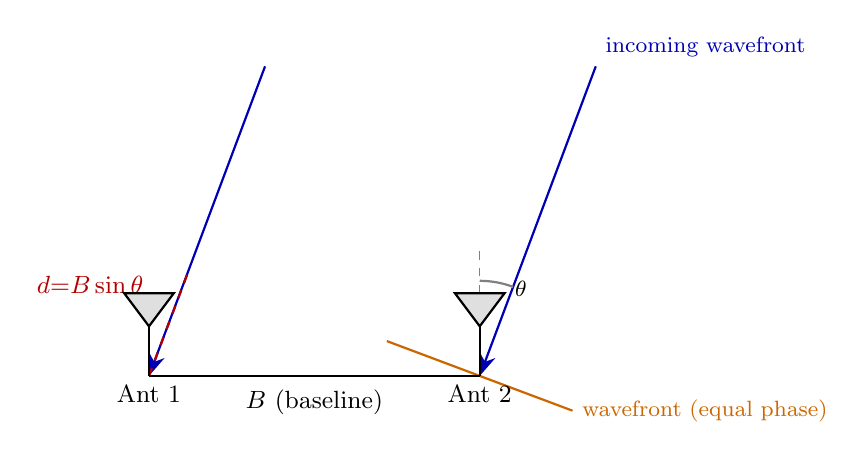
\begin{tikzpicture}[scale=1.05, every node/.style={font=\small}]
% Antennas
\coordinate (A1) at (0,0);
\coordinate (A2) at (4,0);

% incoming ray arrows (parallel)
\draw[-{Stealth[length=8pt]}, blue!70!black, thick] (1.404,3.744) -- (A1);
\draw[-{Stealth[length=8pt]}, blue!70!black, thick] (5.404,3.744) -- (A2);
\node[blue!70!black, above right] at (5.404,3.744) {\footnotesize incoming wavefront};

% wavefront line through A2 (perpendicular to ray)
\draw[thick, orange!80!black] (2.877,0.421) -- (5.123,-0.421);
\node[orange!80!black, right] at (5.123,-0.421) {\footnotesize wavefront (equal phase)};

% baseline
\draw[thick] (A1) -- (A2);
\node[below] at (2,-0.05) {$B$ (baseline)};

% extra path (dashed, from A1 to foot of perpendicular)
\draw[dashed, thick, red!70!black] (A1) -- (0.496,1.314);
\node[red!70!black, left] at (0.05,1.1) {$d{=}B\sin\theta$};

% angle theta marker at A2
\draw[dashed, gray] (A2) -- ++(0,1.6);
\draw[gray, thick] (A2) ++(0,1.15) arc[start angle=90, end angle=69.4, radius=1.15];
\node at (4.5,1.05) {\footnotesize $\theta$};

% antenna symbols
\foreach \p in {A1,A2} {
  \draw[thick] (\p) -- ++(0,0.6);
  \draw[thick, fill=gray!25] ($(\p)+(0,0.6)$) -- ++(-0.3,0.4) -- ++(0.6,0) -- cycle;
}
\node[below] at (A1) {Ant~1};
\node[below] at (A2) {Ant~2};
\end{tikzpicture}

\vspace{4pt}
\footnotesize
\textbf{One antenna} sees only power --- no direction. \textbf{Two
antennas} see a path-length difference $d = B\sin\theta$: a phase shift
that becomes a measurable \textbf{fringe} as Earth's rotation sweeps
$\theta$. Van Cittert--Zernike: this fringe pattern $V(u,v)$ \emph{is}
the Fourier transform of the sky brightness $I(l,m)$.
\end{frame}

\begin{frame}{\ftitle{Resolution \& the Jinc Visibility Function}}
\begin{itemize}
  \item \textbf{Angular resolution:} $\theta \approx \lambda / B_{\max}$ ---
  longer baselines resolve finer sky structure.
  \item \textbf{Fringe period at transit:}
  $T = \dfrac{\lambda}{B\cos\delta\,\omega_E}$
  \item \textbf{Uniform-disk visibility (jinc):}
  \[
  |V(b)| = \left|\frac{2J_1(\pi\theta_\odot b/\lambda)}{\pi\theta_\odot b/\lambda}\right|
  \]
  \item[$\Rightarrow$] First null at $B_{\rm null}\approx 1.22\lambda/\theta_\odot
  \approx 130$~m (610~MHz, $\theta_\odot{=}0.53^\circ$) --- exactly the
  baseline scale where Case~2's 130~m array starts to resolve the solar disk.
\end{itemize}
\end{frame}

\begin{frame}{\ftitle{Aperture Synthesis Imaging}}
\begin{itemize}
  \item $(u,v,w)$: baseline expressed in wavelengths --- the spatial-frequency
  coordinate sampled by the array as the Earth rotates.
  \item Inverting the sampled visibilities by a Fourier transform gives the
  \textbf{dirty image}:
  \[
    I^{D} = I^{\rm sky} \ast B^{D}
  \]
  where $B^D$ is the synthesised beam (point-spread function, PSF).
  \item More/better-distributed baselines $\Rightarrow$ narrower PSF, better resolution.
  \item[$\Rightarrow$] Friis, Johnson--Nyquist, and van Cittert--Zernike ---
  these formulas are exactly the physics implemented at each stage of the
  simulation pipeline, shown next.
\end{itemize}
\end{frame}

% ============================================================
\section{Antenna Design}

\begin{frame}{\ftitle{Antenna: The Yagi-Uda Element}}
\begin{columns}[c]
\column{.48\textwidth}
\centering
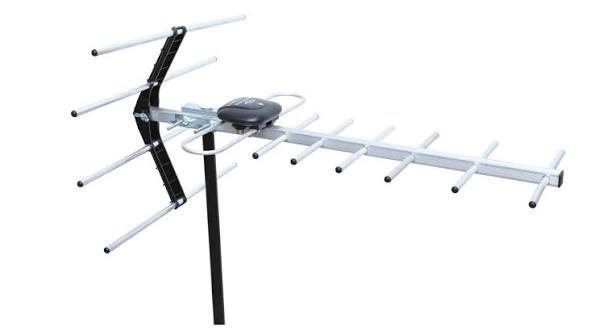
\includegraphics[width=\linewidth]{figs/photo_hkd_antenna.jpg}\\
\small Commercial HKD~G11KD-T2 Yagi-Uda: six directors, U-frame reflector.
\column{.48\textwidth}
\centering
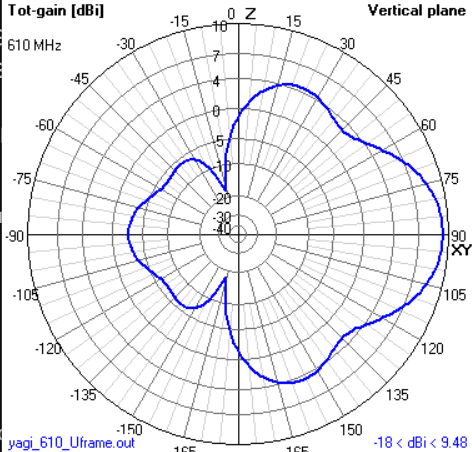
\includegraphics[width=\linewidth]{figs/fig_pattern_eplane_crop.png}\\
\small Simulated E-plane (vertical) pattern, 610~MHz (4NEC2).
\end{columns}
\vspace{4pt}
\begin{itemize}
  \footnotesize
  \item Low-cost, off-the-shelf UHF TV antenna, repurposed as a solar
  radio interferometer element.
  \item Directional gain toward the horizon --- well matched to a
  low-elevation solar transit at Learmonth's latitude.
\end{itemize}
\end{frame}

\begin{frame}{\ftitle{Yagi-Uda Antenna: 4NEC2 Model \& Performance}}
\begin{columns}[c]
\column{.46\textwidth}
\begin{table}
\footnotesize
\begin{tabular}{lc}
\toprule
\textbf{Quantity} & \textbf{Value} \\
\midrule
Input $Z$ & $108.4 - j22.0\;\Omega$ \\
Forward gain & 9.48 dBi \\
HPBW & $\approx 52^\circ$ \\
SWR (75~$\Omega$) & 1.55 \\
\bottomrule
\end{tabular}
\end{table}
\begin{itemize}
  \footnotesize
  \item Commercial folded-dipole Yagi-Uda (6 directors), modelled
  wire-by-wire in 4NEC2~\cite{nec2}.
  \item Real part close to 75~$\Omega$ coax $\Rightarrow$ good match
  without a balun network.
\end{itemize}
\column{.5\textwidth}
\centering
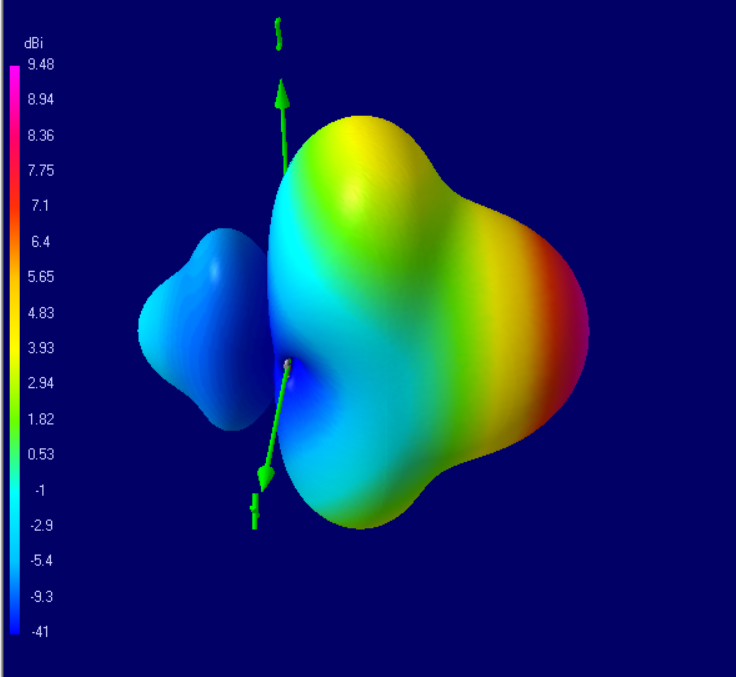
\includegraphics[width=\linewidth]{figs/fig_3d_radiation_pattern.png}\\
\small 3-D directivity pattern at 610~MHz.
\end{columns}
\end{frame}

\begin{frame}{\ftitle{Hardware Validation \& Mutual Coupling}}
\begin{columns}[c]
\column{.44\textwidth}
\begin{table}
\footnotesize
\centering
\begin{tabular}{lcc}
\toprule
\textbf{Method} & \textbf{SWR} & \makecell{\textbf{Return}\\\textbf{loss}} \\
\midrule
NanoVNA & 1.59 & $\approx-12.8$~dB \\
4NEC2   & 1.55 & $\approx-13.3$~dB \\
\bottomrule
\end{tabular}
\end{table}
\begin{itemize}
  \footnotesize
  \item Measured and simulated impedance agree within a narrow range ---
  the simulated pattern is trustworthy enough to drive the imaging pipeline.
\end{itemize}
\column{.52\textwidth}
\centering
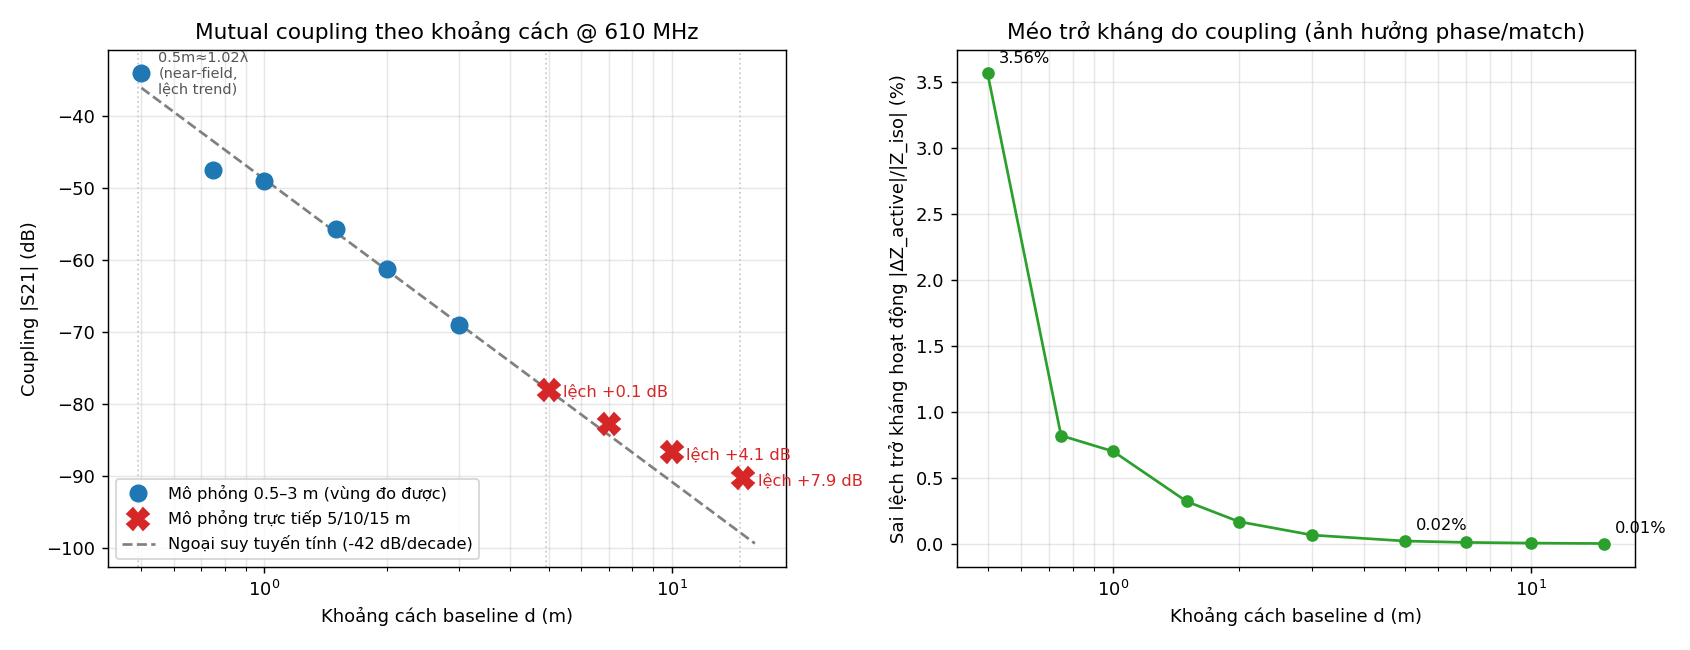
\includegraphics[width=\linewidth]{figs/fig_coupling_curve.png}
\begin{itemize}
  \footnotesize
  \item Coupling falls below $-78$~dB by 5~m and $-87$~dB by 10~m
  $\Rightarrow$ antennas behave as \textbf{independent sensors} at the
  operating baselines used in this thesis (8~m and above).
\end{itemize}
\end{columns}
\end{frame}

% ============================================================
\section{Simulation Pipeline}

\begin{frame}{\ftitle{Pipeline Overview: Engine A --- Voltage Synthesis}}
\centering
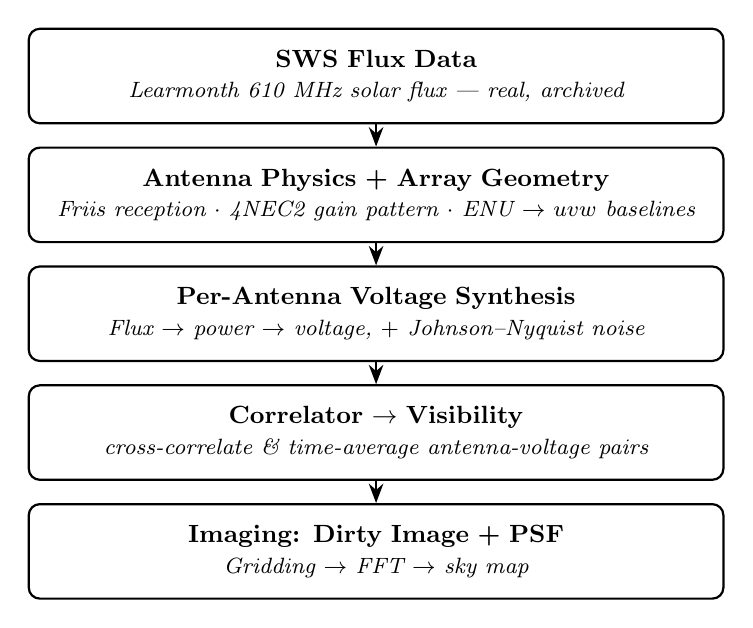
\begin{tikzpicture}[
  proc/.style={rectangle, rounded corners=4pt, draw=black, thick, fill=white,
               text width=8.4cm, align=center, inner sep=6pt, minimum height=1.2cm,
               font=\small},
  arr/.style={-{Stealth[length=7pt]}, thick}
]
\node[proc] (data) {\textbf{SWS Flux Data}\\{\footnotesize\itshape Learmonth 610~MHz solar flux --- real, archived}};
\node[proc, below=8pt of data] (phys) {\textbf{Antenna Physics + Array Geometry}\\{\footnotesize\itshape Friis reception $\cdot$ 4NEC2 gain pattern $\cdot$ ENU $\to uvw$ baselines}};
\node[proc, below=8pt of phys] (volt) {\textbf{Per-Antenna Voltage Synthesis}\\{\footnotesize\itshape Flux $\to$ power $\to$ voltage, $+$ Johnson--Nyquist noise}};
\node[proc, below=8pt of volt] (corr) {\textbf{Correlator $\to$ Visibility}\\{\footnotesize\itshape cross-correlate \& time-average antenna-voltage pairs}};
\node[proc, below=8pt of corr] (img) {\textbf{Imaging: Dirty Image + PSF}\\{\footnotesize\itshape Gridding $\to$ FFT $\to$ sky map}};
\draw[arr] (data) -- (phys);
\draw[arr] (phys) -- (volt);
\draw[arr] (volt) -- (corr);
\draw[arr] (corr) -- (img);
\end{tikzpicture}
\end{frame}

\begin{frame}{\ftitle{Engine B: Analytic Cross-Check \& Jinc Validation}}
\begin{columns}[c]
\column{.4\textwidth}
\centering
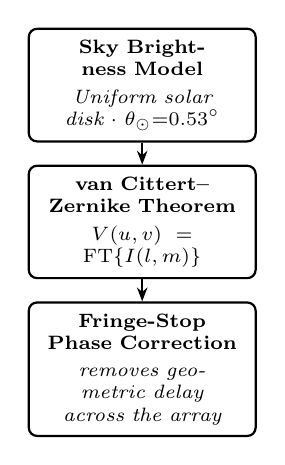
\begin{tikzpicture}[
  proc/.style={rectangle, rounded corners=3pt, draw=black, thick, fill=white,
               text width=2.6cm, align=center, inner sep=4pt, minimum height=1.3cm,
               font=\scriptsize},
  arr/.style={-{Stealth[length=5pt]}, thick}
]
\node[proc] (sky) {\textbf{Sky Brightness Model}\\[2pt]{\itshape Uniform solar disk $\cdot$ $\theta_\odot{=}0.53^\circ$}};
\node[proc, below=8pt of sky] (vcz) {\textbf{van Cittert--Zernike Theorem}\\[2pt]{\itshape $V(u,v) = \mathrm{FT}\{I(l,m)\}$}};
\node[proc, below=8pt of vcz] (fs) {\textbf{Fringe-Stop Phase Correction}\\[2pt]{\itshape removes geometric delay across the array}};
\draw[arr] (sky) -- (vcz);
\draw[arr] (vcz) -- (fs);
\end{tikzpicture}
\column{.56\textwidth}
\centering
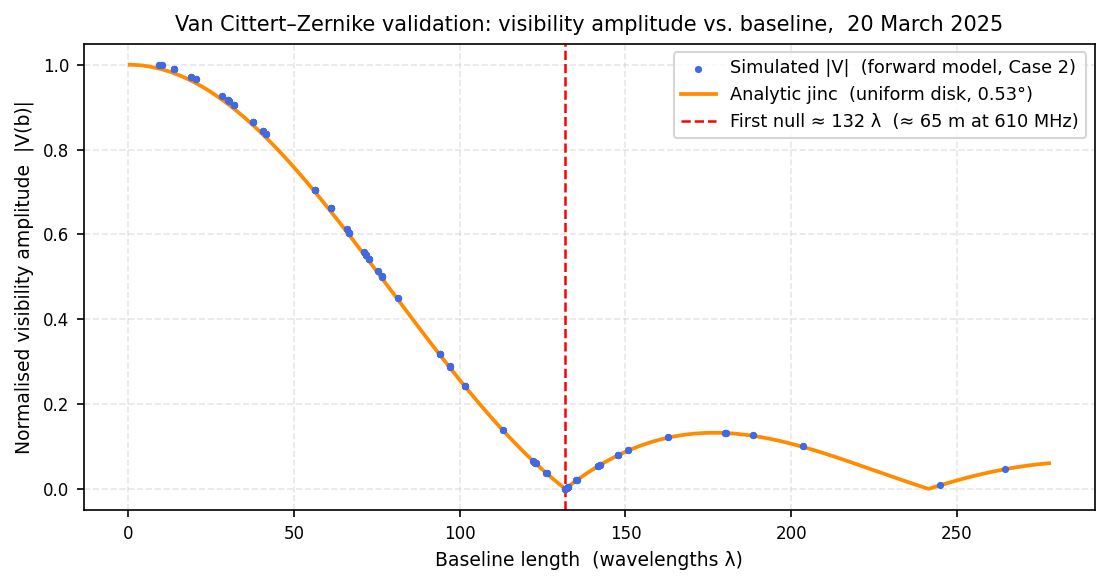
\includegraphics[width=\linewidth]{figs/fig_visibility_jinc.png}
\end{columns}
\vspace{4pt}
\begin{itemize}
  \footnotesize
  \item Fast, closed-form analytic model --- \emph{not} a full per-antenna
  signal chain; used only to cross-check Engine A.
  \item \textbf{Validation:} visibility amplitude decays as
  $\jinc(u\,\theta_\odot)$ with baseline length, matching Engine A's
  correlator output at transit peak.
\end{itemize}
\end{frame}

\begin{frame}{\ftitle{Input Data \& Voltage Synthesis}}
\centering
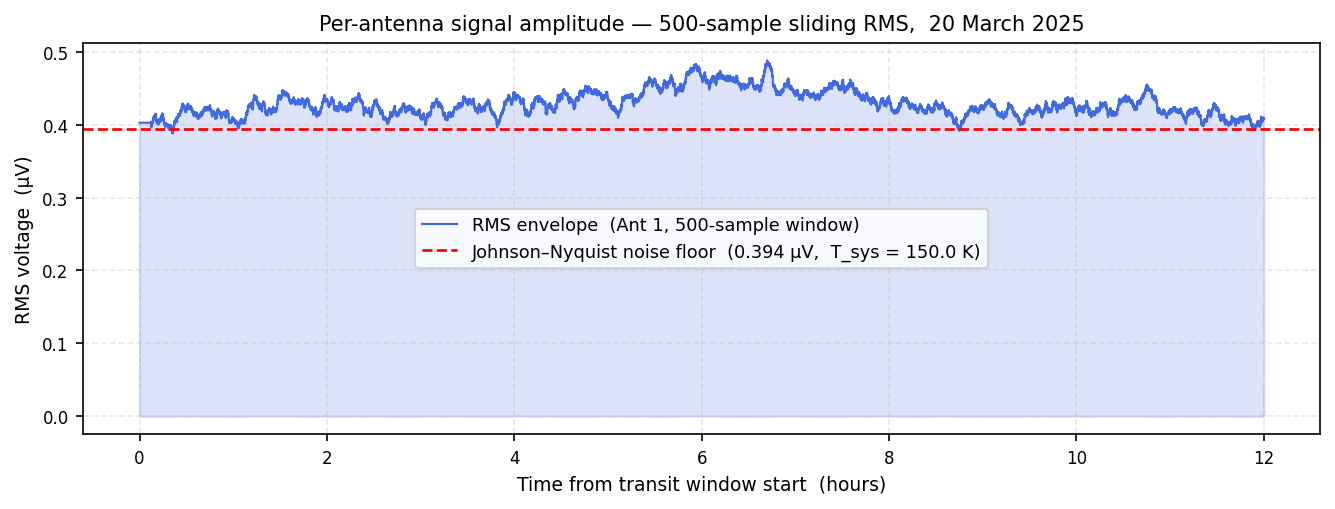
\includegraphics[width=0.85\linewidth]{figs/fig_voltage_env.png}

\vspace{4pt}
\begin{itemize}
  \footnotesize
  \item Real, archived, already-calibrated 610~MHz flux from SWS
  Learmonth, Australia~\cite{sws} (20 March 2025, spring equinox) drives
  the whole chain --- not re-simulated internally.
  \item Flux $\to$ Friis power $\to$ voltage, with additive
  Johnson-Nyquist noise and the 4NEC2 primary beam applied along the
  solar track.
  \item Output: per-antenna complex baseband voltage, ready for correlation.
\end{itemize}
\end{frame}

\begin{frame}{\ftitle{Array Geometry \& Imaging Validation}}
\centering
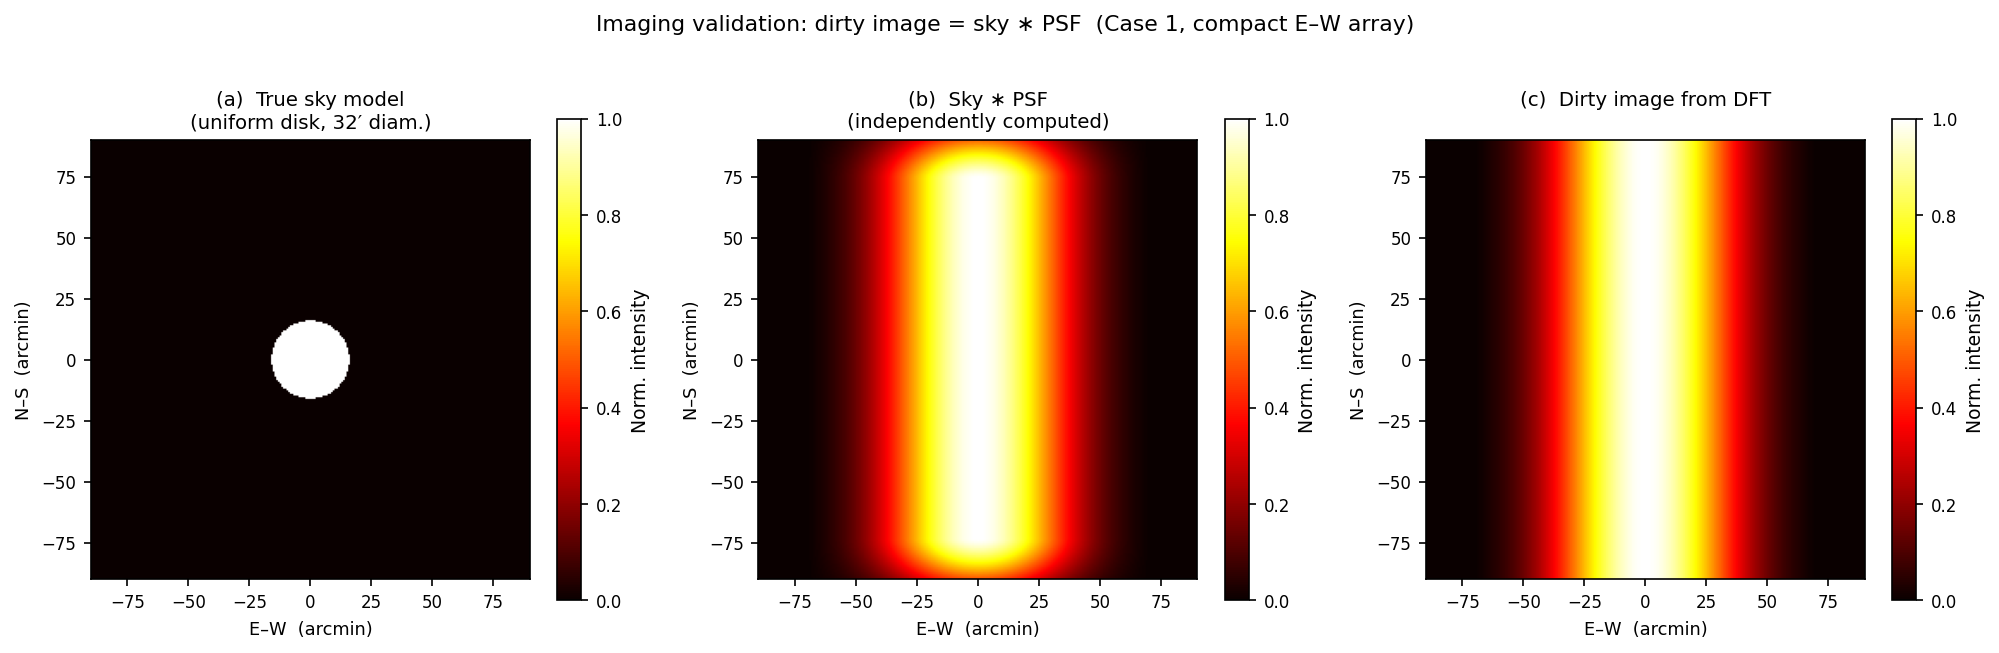
\includegraphics[width=0.85\linewidth]{figs/fig_sky_conv_psf.png}
\begin{itemize}
  \footnotesize
  \item One consistent ENU$\to$XYZ$\to uvw$ geometry transform works for
  \emph{any} 2-D array layout --- key to comparing configurations fairly.
  \item The \textbf{dirty image} is the true sky convolved with the
  array's \textbf{point-spread function (PSF)}, $I^D=I^{\rm sky}\ast B^D$
  (panels a+b); sidelobes come from incomplete $uv$-sampling, not real
  structure.
  \item Panel (c), computed independently via gridding + FFT, agrees with
  (b) --- validating the imaging stage.
\end{itemize}
\end{frame}

% ============================================================
\section{Evaluation \& Results}

\begin{frame}{\ftitle{Two Kinds of Results}}
\begin{columns}[c]
\column{.48\textwidth}
\begin{block}{Track A --- Data Reproduction}
\footnotesize
\emph{Does the simulator match reality?}
\begin{itemize}
  \item Jinc visibility vs.\ baseline: matches analytic theory exactly.
  \item Solar excess vs.\ real Hoa Lac hardware: SNR gap fully explained.
\end{itemize}
\end{block}
\column{.48\textwidth}
\begin{alertblock}{Track B --- Design Simulation}
\footnotesize
\emph{Given a trustworthy simulator, which antenna placement is best?}
\begin{itemize}
  \item Cases 1, 1.5, 1.75, 2: same handful of antennas, different
  \textbf{geometry} --- simulated only, none yet built.
\end{itemize}
\end{alertblock}
\end{columns}
\vspace{6pt}
\begin{table}
\footnotesize
\centering
\begin{tabular}{lll}
\toprule
\textbf{Case} & \textbf{Layout} & \textbf{Track} \\
\midrule
1    & Compact E-W, 4 ant.\ (24~m)     & B: baseline (1-D only) \\
1.5  & Cross, 4 ant.\ (8~m unit)       & B: recover 2-D resolution \\
1.75 & DLITE-inspired triangle+centre  & B: non-redundant, minimal-antenna 2-D \\
2    & Extended graded cross (130~m)  & B: resolve the solar disk \\
\bottomrule
\end{tabular}
\end{table}
\centering
\textbf{Track A earns trust in the tool; Track B is what the tool is
\emph{for}.}
\end{frame}

\begin{frame}{\ftitle{Case 1: Compact E-W Array}}
\centering
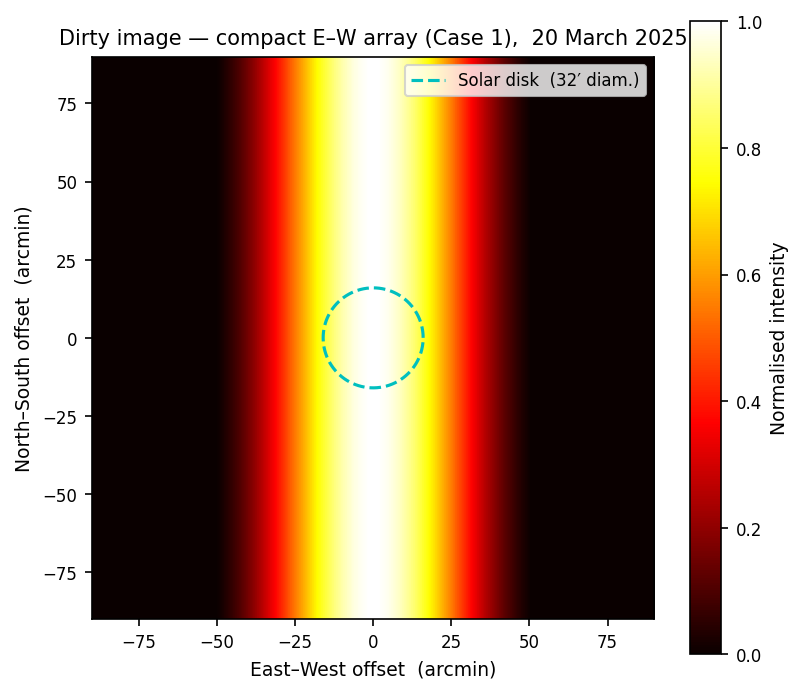
\includegraphics[width=0.48\linewidth]{figs/fig_dirty_image.png}
\begin{itemize}
  \item Compact 4-antenna E-W line (24~m total) --- \textbf{1-D baselines only}.
  \item Dirty image is sharp in E-W ($\sim35'$ FWHM) but the source is
  completely \textbf{smeared in N-S} ($180'$ FWHM --- effectively
  unresolved): no baseline component senses that direction.
  \item[$\Rightarrow$] A 1-D array cannot recover a 2-D image.
\end{itemize}
\end{frame}

\begin{frame}{\ftitle{Case 1.5: Cross Layout Recovers 2-D Resolution}}
\centering
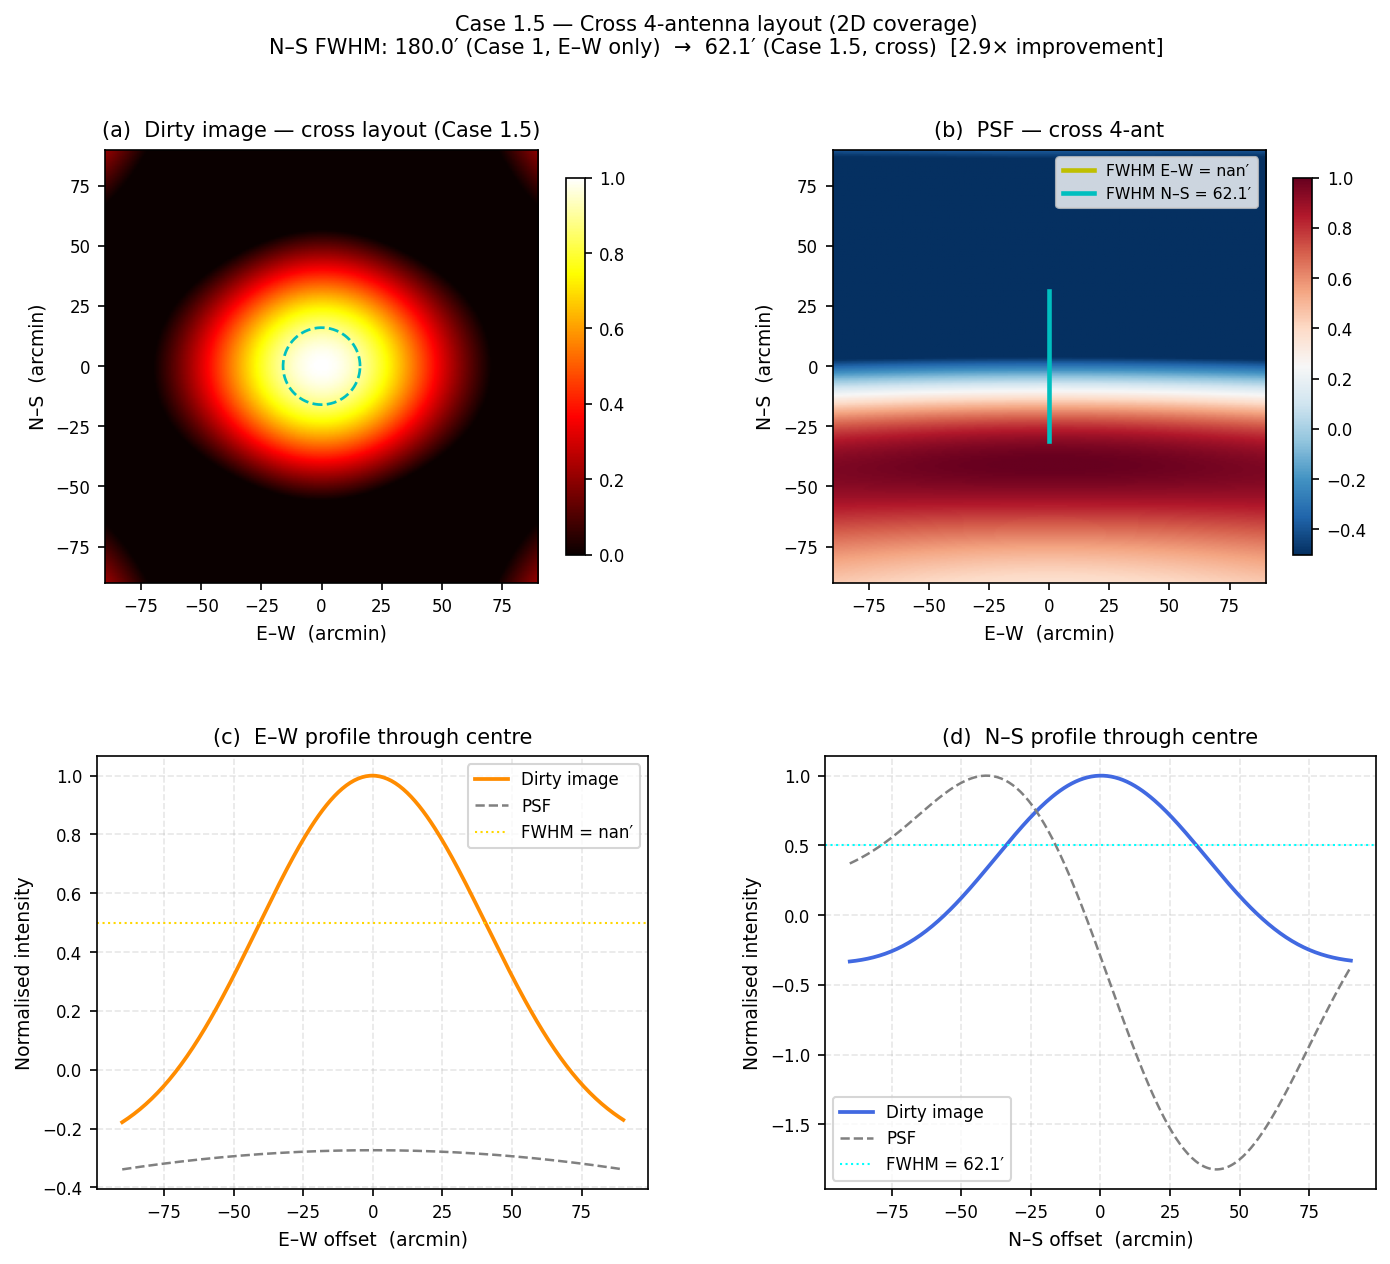
\includegraphics[width=0.4\linewidth]{figs/fig_dirty_from_dft.png}
\begin{table}
\footnotesize
\centering
\begin{tabular}{lcc}
\toprule
\textbf{Layout} & FWHM N-S & Improvement \\
\midrule
Case 1 (E-W only) & $180.0'$ & --- \\
Case 1.5 (Cross)  & $62.1'$  & $2.9\times$ \\
\bottomrule
\end{tabular}
\end{table}
\begin{itemize}
  \footnotesize
  \item Same 4 antennas, rearranged into a \textbf{cross} (adds a N-S arm)
  --- same hardware, better geometry.
  \item[$\Rightarrow$] N-S resolution recovers substantially, but the
  cross is not yet fully symmetric --- Case~1.75 pushes this further.
\end{itemize}
\end{frame}

\begin{frame}{\ftitle{Case 1.75: DLITE-Inspired Layout}}
\begin{columns}[c]
\column{.36\textwidth}
\centering
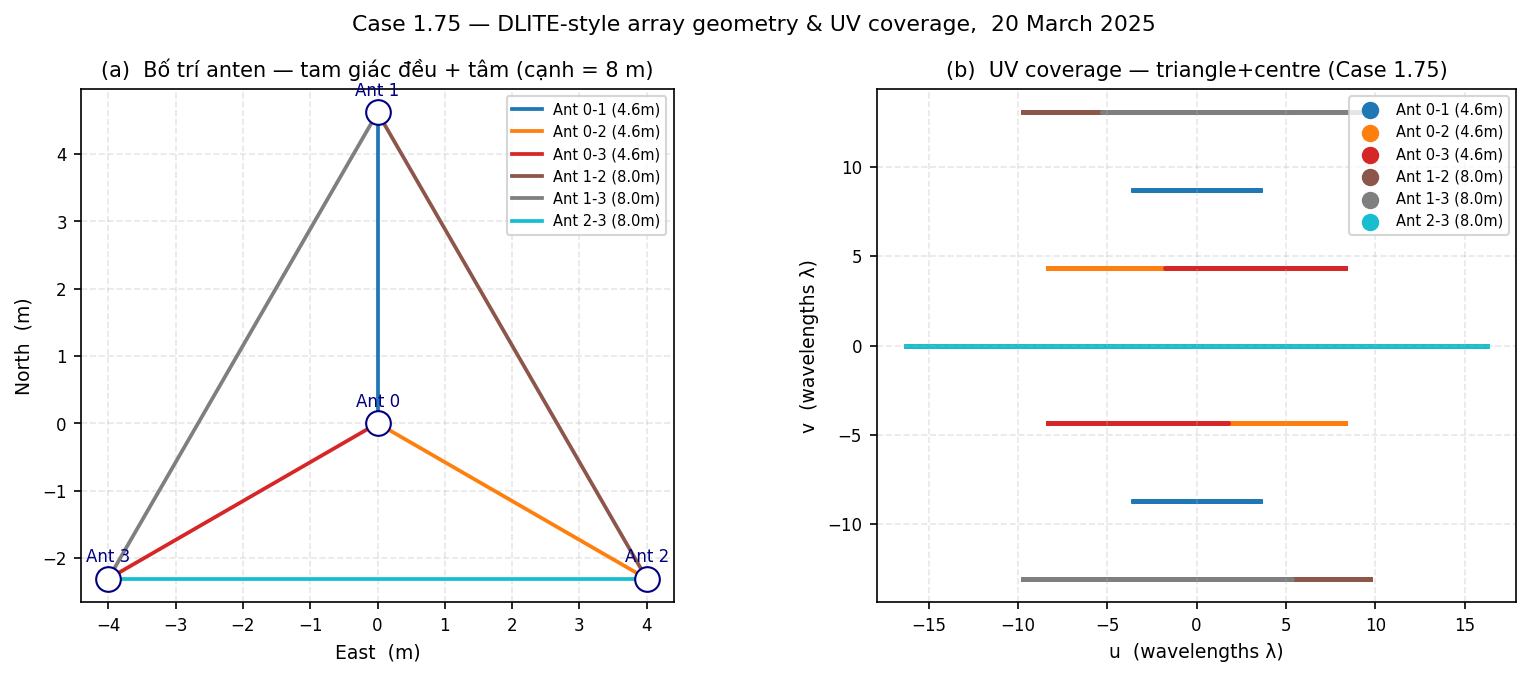
\includegraphics[width=\linewidth]{figs/fig_case175_geometry.png}
\column{.52\textwidth}
\centering
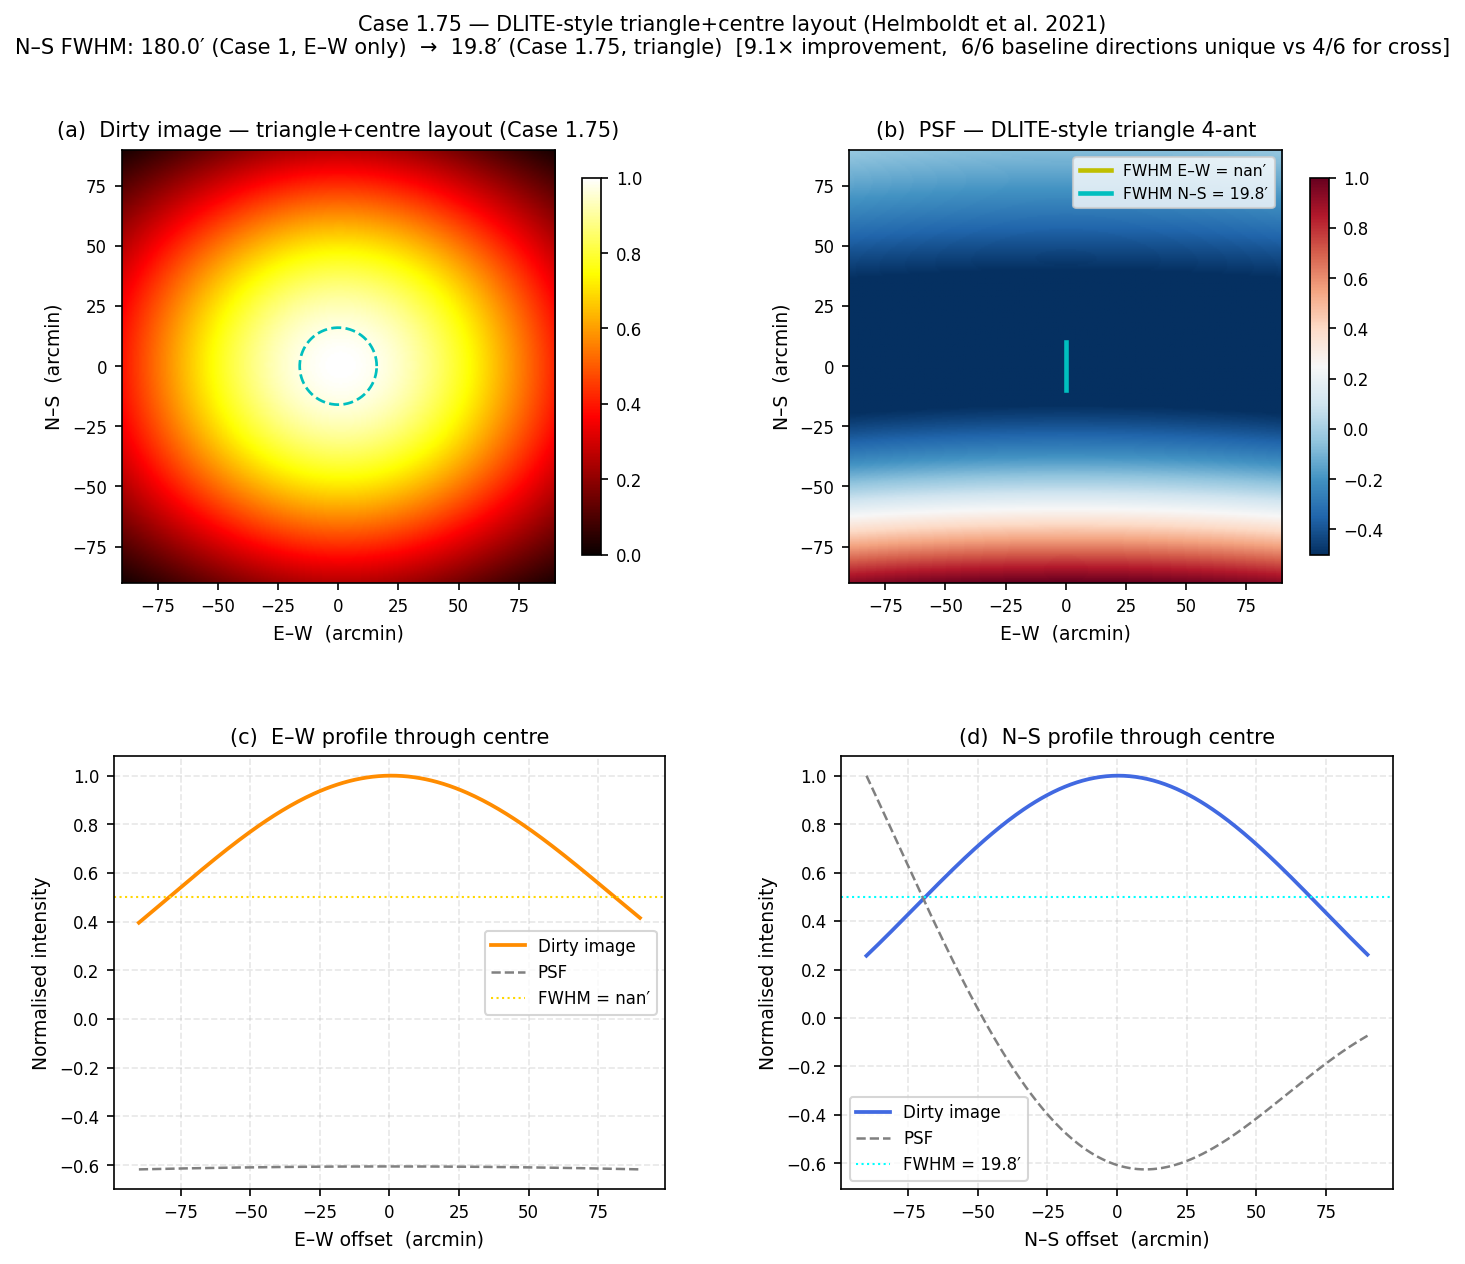
\includegraphics[width=\linewidth]{figs/fig_case175_eval.png}
\end{columns}
\vspace{2pt}
\footnotesize
\begin{itemize}
  \item Same four antennas, same 8~m spacing --- rearranged as a triangle plus
  a centre element, inspired by DLITE's minimum-redundancy
  philosophy~\cite{helmboldt2021dlite}.
  \item All six baselines point in \textbf{distinct} directions $\Rightarrow$
  North-South FWHM improves \textbf{9.1$\times$} versus Case~1.
  \item Not a full DLITE simulation: same topology, but at 610~MHz with an
  8~m scale, not DLITE's 30--40~MHz / hundreds-of-metres system.
\end{itemize}
\end{frame}

\begin{frame}{\ftitle{Case 2: Resolving the Solar Disk}}
\centering
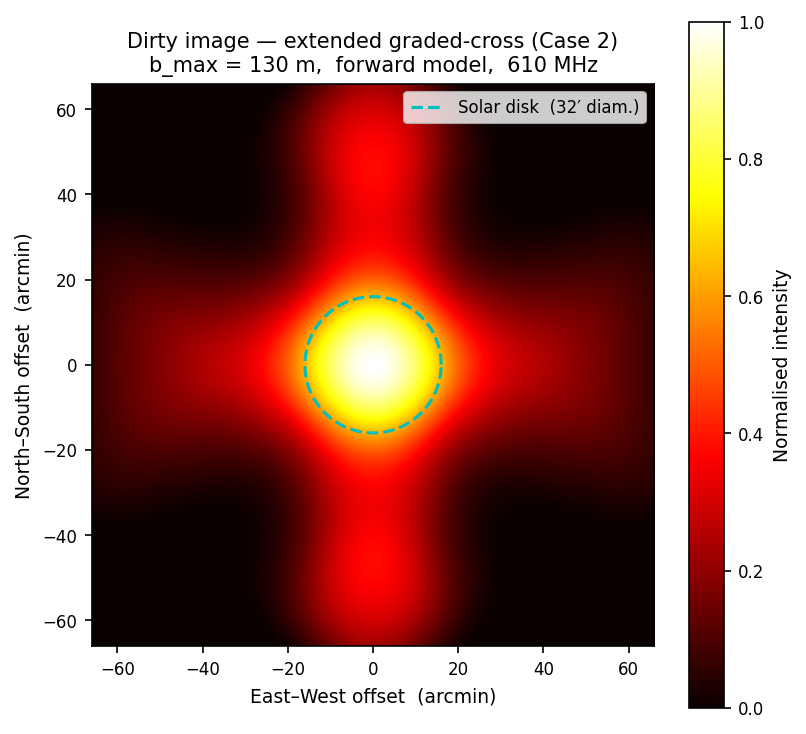
\includegraphics[width=0.5\linewidth]{figs/fig_case2_image.png}
\begin{itemize}
  \item Extended graded-cross array, baselines up to 130~m
  ($u_{\rm max}\approx 265\,\lambda$).
  \item E-W resolution $\approx 11'$ --- sufficient to begin resolving the
  $32'$ solar disk.
  \item Visibility amplitude drops below 50\% by $u\approx130\,\lambda$: the
  interferometric signature of a partially resolved source.
\end{itemize}
\end{frame}

\begin{frame}{\ftitle{Array Geometry Comparison Matrix}}
\begin{table}
\footnotesize
\centering
\begin{tabular}{lccc}
\toprule
\textbf{Layout} & \textbf{Max baseline} & \textbf{N-S FWHM} & \textbf{vs.\ Case~1} \\
\midrule
Case 1 (E-W line)       & 24~m  & $180.0'$ (smeared) & --- \\
Case 1.5 (Cross)        & 8~m   & $62.1'$             & $2.9\times$ \\
\rowcolor{yellow!25}
Case 1.75 (DLITE triangle) & 8~m & $19.8'$            & $\mathbf{9.1\times}$ \\
Case 2 (Extended cross) & 130~m & $\approx11'$ (E-W)  & resolves disk \\
\bottomrule
\end{tabular}
\end{table}
\begin{itemize}
  \item[$\Rightarrow$] \textbf{Takeaway:} Case~1.75 uses the \emph{same}
  8~m spacing as Case~1.5 --- rearranging the \emph{same} antennas beats
  blindly adding more hardware in a bad geometry. \textbf{Placement, not
  antenna count, is the lever that matters.}
\end{itemize}
\end{frame}

\begin{frame}{\ftitle{Sensitivity \& Burst Detectability}}
\begin{itemize}
  \item Quiet-Sun signal alone reaches SNR $\approx 1{,}700$ per integration dump.
  \item Every burst category in the catalogue is detectable at extreme significance:
\end{itemize}
\begin{table}
\footnotesize
\centering
\begin{tabular}{lcc}
\toprule
\textbf{Event type} & \textbf{Flux (sfu)} & \textbf{SNR (1 dump)} \\
\midrule
Quiet Sun         & --              & $\approx 1{,}700$ \\
Type IV continuum & $\sim$200--1{,}000 & 3{,}400--17{,}200 \\
Type III (moderate) & $\sim$1{,}000 & $\sim$17{,}200 \\
Type II (shock)   & 500--5{,}000    & 8{,}600--86{,}000 \\
\bottomrule
\end{tabular}
\end{table}
\end{frame}

\begin{frame}{\ftitle{Answering the Black-Box Problem}}
\begin{itemize}
  \item Simulated solar excess compared against the two-element analogue
  interferometer at Hoa Lac, Hanoi (20 March 2025, same transit date).
  \item A factor of \textbf{23.8$\times$} gap in SNR is found, attributed to
  the high effective system temperature of the consumer SDR receiver
  ($T_{\rm sys,eff}\approx 3{,}600$~K vs.\ the ideal $150$~K model).
\end{itemize}
\begin{alertblock}{Verdict, revisiting the Section~1 checklist}
Of the four candidate causes (phase-incoherent oscillators, cable loss,
RFI, thermal noise), simulation confirms the dominant one is
\textbf{system temperature} --- not signal-chain modelling, not
geometry. \cmark\ Black box solved; the other three causes are ruled out
as dominant.
\end{alertblock}
\end{frame}

\begin{frame}{\ftitle{Tools: APSYNSIM \& Companion Simulator}}
\begin{columns}[c]
\column{.42\textwidth}
\begin{itemize}
  \footnotesize
  \item \textbf{APSYNSIM}~\cite{apsynsim}: widely-used open-source
  aperture-synthesis teaching tool (Onsala) --- synthetic sky, simplified
  Gaussian beam, no real flux or hardware pattern.
  \item[$\Rightarrow$] This work adds real Learmonth flux, a measured
  4NEC2 antenna pattern, and a real hardware comparison --- at the cost of
  being tied to one physical scenario.
\end{itemize}
\column{.54\textwidth}
\centering
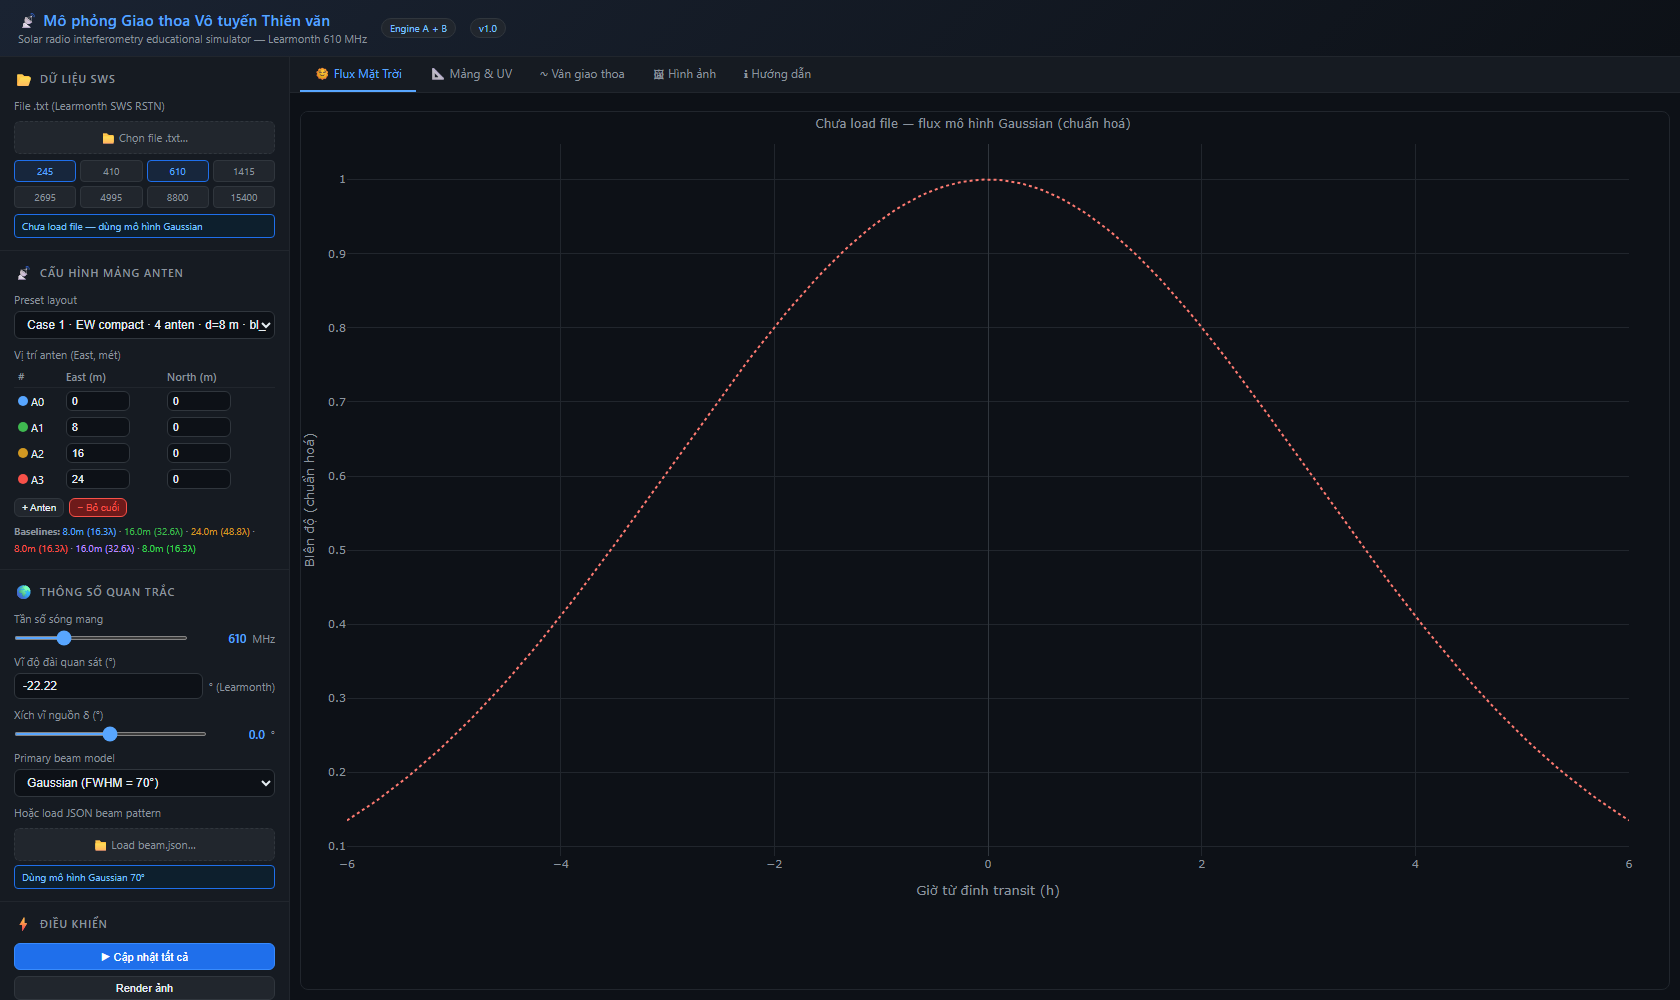
\includegraphics[width=\linewidth]{figs/fig_html_tool_main.png}\\
\footnotesize Companion \texttt{radio\_simulation.html}: browser-based,
Case~1--5 presets, live sliders, no Python required.
\end{columns}
\end{frame}

% ============================================================
\section{Conclusion \& Future Work}

\begin{frame}{\ftitle{Objectives Revisited: Are We Done?}}
\begin{block}{\cmark\ 1. Build a trustworthy physics simulator}
\footnotesize
4NEC2 antenna model cross-checked against direct NanoVNA measurement;
jinc visibility matches analytic theory exactly; Hoa Lac hardware
comparison explains the 23.8$\times$ SNR gap --- \textbf{Black-Box
Problem solved} (system temperature, not geometry or signal chain).
\end{block}
\vspace{4pt}
\begin{block}{\cmark\ 2. Optimize antenna placement}
\footnotesize
Same 4-antenna hardware, four geometries tested: E-W line
$\to$ cross $\to$ DLITE-inspired triangle gives a
\textbf{9.1$\times$} N-S resolution gain from \emph{rearrangement alone};
extended cross (Case~2) begins resolving the $32'$ solar disk.
\end{block}
\vspace{4pt}
\begin{itemize}
  \footnotesize
  \item Bonus: a reproducible single-notebook workflow (raw flux $\to$
  calibrated dirty image, under two minutes) and a browser-based
  companion tool for live exploration.
\end{itemize}
\end{frame}

\begin{frame}{\ftitle{Conclusion \& Future Work}}
\begin{itemize}
  \item Space weather and GNSS impacts motivate ground-based solar radio
  monitoring; large dishes are costly, so low-cost interferometry (DLITE,
  and this work) is a realistic alternative.
  \item This thesis shows that a physically grounded, end-to-end
  simulation \emph{can} evaluate feasibility, signal chain, and array
  geometry \textbf{before} further hardware deployment --- turning the
  ambiguous Xuan Mai field result into a specific, addressable list of
  hardware requirements.
\end{itemize}
\begin{block}{Future Work}
\footnotesize
\begin{itemize}
  \item FPGA hardware correlator, hardware-in-the-loop fringe validation.
  \item Physical DLITE-inspired array upgrade at Xuan Mai (triangle + centre).
  \item Recorded Type~II/III burst input; CLEAN
  deconvolution~\cite{hogbom1974}, multi-frequency imaging, real-time
  operation, GPS-disciplined clock.
\end{itemize}
\end{block}
\end{frame}

% ============================================================
\begin{frame}[allowframebreaks]
\frametitle{References}
\tiny{
\bibliography{refs_slides}
}
\end{frame}

\begin{frame}
\Huge{\centerline{Thank you!}}
\end{frame}

\end{document}
